% Active Localization -- 2-page report (T-012a skeleton, T-012b: RND review 05_report_review.md applied).
% Build: report/build.sh  (latexmk + pdflatex) -> report/report.pdf, must be <= 2 pages.
%
% Source convention: every number in the text carries a comment `% src: <file>`.
%   _team/...  = team bus (DECISIONS, FACTS, tasks, knowledge/rnd)
%   repo paths = relative to the repository root
% Parameter values follow _team/tasks/T-009_method_impl.md v2 (RND-7) and the
% active Nav2 params used in the runs (navigation/src/nav2_planner_custom/config/nav2_params_active.yaml).
% T-012e: sections 5-6 = RND's final text (_team/knowledge/rnd/08_final_findings.md §3, T-011 final);
% results from T-010b (runs/t010b_20261019_055924/{x4,x6}) and D-6 (runs/d6_20261019_055924).
% Local copies of the inputs: _team/final_inputs/ (08_final_findings.md, 07_results_draft.md,
% T-010b_ENG.md, summary_x4.md, summary_x6.md, summary_table.tex, trajectories.pdf, paired_t010b.pdf).
% The only remaining red TODO is DIR's title block (authors, affiliation, date, repo link, subtitle).
\documentclass[10pt,twocolumn]{article}
\usepackage[a4paper,margin=1.5cm,columnsep=0.6cm]{geometry}
\usepackage[T1]{fontenc}
\usepackage{mathptmx}
\usepackage{amsmath,amssymb}
\usepackage{graphicx}
\usepackage{booktabs}
\usepackage{tabularx}
\usepackage{xcolor}
\usepackage{tikz}
\usetikzlibrary{positioning,arrows.meta,fit}
\usepackage[font=footnotesize,labelfont=bf,skip=3pt]{caption}
\usepackage[compact]{titlesec}
\usepackage{enumitem}
\usepackage{microtype}
\usepackage[hidelinks]{hyperref}

\titleformat{\section}{\normalsize\bfseries}{\thesection}{0.5em}{}
\titlespacing*{\section}{0pt}{5pt plus 1pt}{2pt}
\setlist{nosep,leftmargin=1.1em}
\setlength{\abovedisplayskip}{3pt}\setlength{\belowdisplayskip}{3pt}
\setlength{\abovedisplayshortskip}{2pt}\setlength{\belowdisplayshortskip}{2pt}
\setlength{\textfloatsep}{6pt}\setlength{\floatsep}{6pt}
\setlength{\parskip}{0pt}

\newcommand{\TODO}[1]{\textcolor{red}{\textbf{TODO:} #1}}

\title{\vspace{-1.2cm}\large\bfseries Active Localization in Nav2: Steering Heading and Route toward Fiducial Landmarks\\[-2pt]
  {\normalsize\mdseries an analytic, FIF-inspired scorer with ActLoc-style heading planning and a RAVPP-style route layer}\vspace{-0.3cm}}
% subtitle: RND suggestion (05_report_review.md #15), DIR to confirm
\author{\small \TODO{authors, affiliation, date, repository link; confirm subtitle (DIR)}}
\date{\vspace{-0.9cm}}

\begin{document}
\maketitle

% =====================================================================
\section{Problem and testbed}
% =====================================================================
An omnidirectional Astribot base in Gazebo localizes with RTAB-Map from 360\textdegree{} lidar ICP plus five STag HD17 fiducials used as landmarks (ids 1--5), and navigates with stock Nav2 (Theta* + MPPI Omni), which drives \emph{facing forward}.
% src: _team/knowledge/FACTS.md (16.10: planar_move omni, RTAB-Map lidar ICP + HD17 ids 1-5, Nav2 Theta* + MPPI forward_preference)
The only camera is rigidly mounted on the torso (640$\times$480, HFOV 1.089\,rad), so the robot's heading is its gaze, and an omni base can choose that heading freely along any path.
% src: _team/knowledge/FACTS.md (16.10 camera torso_rgbd; 18.10 camera mount)
All markers sit on two shelf rows ($y\approx0.9$ and $3.4$\,m) and face $-y$; a marker is detected only if its projected area $A=(fs/r)^2\cos\theta\ge{\approx}500$\,px$^2$, i.e.\ $r\le 1.88\sqrt{\cos\theta}$\,m, and $r>r_{\min}\in(0.61,0.71]$\,m.
% src: _team/knowledge/FACTS.md (17.10 landmark export; 18.10 empirical HD17 visibility model, A_min in (485, 508) px^2, r_min in (0.61, 0.71] m)
The task is to plan \emph{where to look} and \emph{which way to drive} so that the localization error w.r.t.\ ground truth decreases compared with the baseline.

% =====================================================================
\section{Method}
% =====================================================================
\textbf{Two levers} (ADR-001, Option 2): the \emph{yaw} along the planned path and the \emph{route} itself. Both are driven by one pose score $s(x,y,\psi)$.
For a bearing measurement with the pose perturbed in the world frame, the information of a \emph{visible} landmark does not depend on the camera heading (FIF, eq.~15); heading acts only through visibility. Hence the score depends on $\psi$ only through the gates in eq.~(1).
% src: _team/DECISIONS.md (ADR-001); _team/knowledge/rnd/02_RESEARCH_iter2_math.md §2.1 (psi not in J, FIF eq. 15)

\textbf{Scorer S2*.} For marker $i$ at $p_i$ with normal $n_i$ and camera centre $c$: $\Delta_i=p_i-c$, $r_i=\|\Delta_i\|$, bearing $\beta_i=\mathrm{wrap}(\mathrm{atan2}(\Delta_{i,y},\Delta_{i,x})-\psi)$, $\cos\theta_i=(-\Delta_i\cdot n_i)/r_i$, $A_i=(f s/r_i)^2\max(\cos\theta_i,0)$:
% src: _team/tasks/T-009_method_impl.md §1
\begin{align}
w_i&=\sigma\!\big(k_{\mathrm{fov}}(\tfrac{\mathrm{HFOV}}{2}-|\beta_i|)\big)\,
    \sigma\!\big(k_A(\tfrac{A_i}{A_{\min}}-1)\big)\nonumber\\
   &\quad\cdot\sigma\!\big(k_r(r_i-r_{\min})\big)\,\mathrm{occ}_i,\nonumber\\
n_{\mathrm{eff}}&=\textstyle\sum_i w_i,\qquad s(x,y,\psi)=1-\exp(-n_{\mathrm{eff}}/M),
\end{align}
% src: _team/tasks/T-009_method_impl.md §2
with $\sigma(z)=1/(1+e^{-z})$ and the values in Table~\ref{tab:params}; $\mathrm{occ}_i=0$ if the segment $c\to p_i$ hits the static map (last 0.20\,m ignored).
% src: _team/tasks/T-009_method_impl.md §1, §2 (v2)
\emph{Why a soft count:} RTAB-Map weights every landmark with a fixed isotropic variance (0.05\,m$^2$), so, with the heading known from lidar/odometry, the position Fisher information is $(\sum_i w_i)/0.05\cdot I$ and det, $\lambda_{\min}$ and trace all reduce to $n_{\mathrm{eff}}$. Physically (bearing/PnP FIM, 1\,px), information falls as $1/r^2$ and, for a small marker, the range error grows as $\sigma_\parallel=r^2\sigma_{\mathrm{px}}/(fs)$: 2.4\,cm at 1\,m, 8.4\,cm at the detection limit (1.88\,m), below the 22\,cm RTAB-Map assumes, so every detected marker can be trusted and only \emph{whether} it is detected matters.
% src: _team/knowledge/rnd/02_RESEARCH_iter2_math.md §3 C1 (S1 sigma_par = d^2 spx/(f s): 2.4 cm at 1 m; RTAB 22.4 cm; marginal yaw info of one marker = 1/sigma_a^2 only), C4 (conditional block), "C2 update after ENG-10" (8.4 cm at 1.88 m); FACTS.md 16.10 (landmark_linear_variance 0.05)
$M=1$ because usually at most one marker is in view.
% src: _team/DECISIONS.md (ADR-001), 02_RESEARCH_iter2_math.md C2 update (d)

\textbf{Route lever: costmap layer.} Best-over-yaw score $s^*(x,y)=\max_{\psi\in\{-\pi+2\pi k/36\}}s(x,y,\psi)$ and
\begin{equation}
\mathrm{cost}(x,y)=\mathrm{round}\big(c_{\max}\,(1-\min(s^*/s_{\mathrm{ref}},1))^p\big),
\end{equation}
$s_{\mathrm{ref}}=1-e^{-1}\approx0.632$, $p=1$, $c_{\max}=150$ (of 252), added to the master cost as $\min(\text{master}+\text{cost},252)$ on cells that are not lethal, inscribed or unknown; adding (not $\max$) keeps the inflation gradient below $c_{\max}$, so paths do not hug the shelves. Theta* then prefers the low-cost band in front of the marker rows (grey in Fig.~\ref{fig:results}a) when the detour is cheap.
% src: _team/tasks/T-009_method_impl.md §3 v2 (additive combine, RND-7 item 2); c_max = 150: _team/DECISIONS.md (D-5 log, DIR 2026-10-18 15:45), nav2_params_active.yaml loc_layer.c_max: 150

% Former Fig. 1 (s_star.png, best-over-yaw score map) removed in T-012e to fit 2 pages:
% the same s* field is the grey background of Fig. 1a (trajectories). File kept in report/figures/.

% Fig. 1 (results; "Fig. 3a/3b" in RND's 08 §4), full width; defined here so that it floats to the top of page 2.
\begin{figure*}[t]
\centering
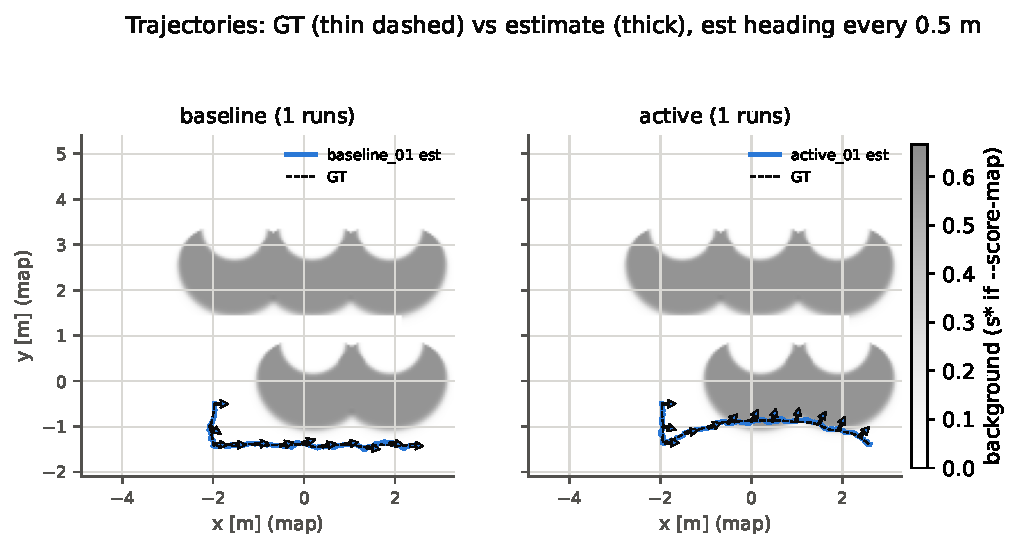
\includegraphics[height=3.5cm,trim=0 0 0 36,clip]{figures/trajectories.pdf}\hfill
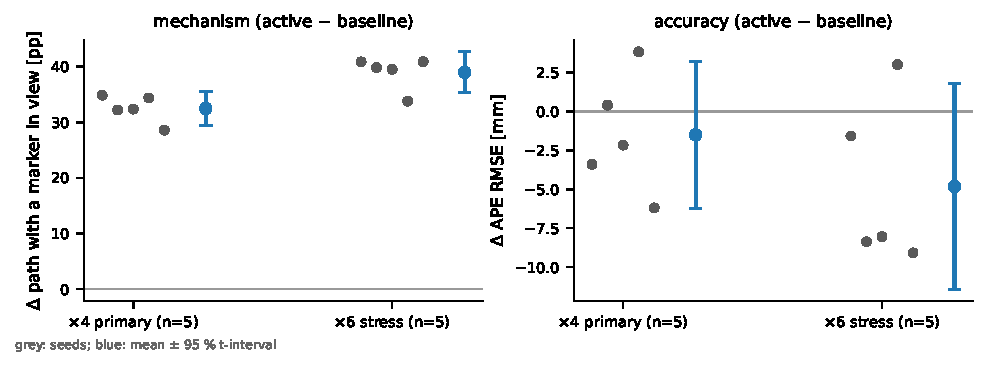
\includegraphics[height=3.5cm]{figures/paired_t010b.pdf}
\caption{(a, left) Route-lever demo (one run): baseline keeps $y=-1.4$\,m and sees no marker; active bends 0.5\,m into the high-$s^*$ band (grey) and faces the markers (arrows). (b, right) Paired differences active $-$ baseline per seed (grey) with mean and 95\,\% $t$-interval (blue).}
% src (a): runs/d6_20261019_055924/plots/trajectories.pdf (_team/final_inputs/trajectories.pdf; suptitle cropped); caption: _team/final_inputs/08_final_findings.md §4
% src (b): knowledge/figures/paired_t010b.pdf (scripts/t011_paired_plot.py; _team/final_inputs/paired_t010b.pdf); 08 §4, 07 §B10
\label{fig:results}
\end{figure*}

\textbf{Yaw lever: heading DP.} The Theta* path is resampled every 0.20\,m and a Viterbi DP over $B=36$ heading bins $\psi_b$ picks one heading per waypoint ($\phi_j$ = travel direction):
% src: _team/tasks/T-009_method_impl.md §4 (step 0.20 m, B = 36)
\begin{gather}
\mathrm{node}(j,b)=-w_s\,\frac{s(x_j,y_j,\psi_b)}{s_{\mathrm{ref}}}+w_f\,(1-\cos(\psi_b-\phi_j)),\nonumber\\
\mathrm{edge}(j,a{\to}b)=w_{sm}\Delta\psi^2+w_{lim}\max(0,|\Delta\psi|-k\,ds_j)^2,
\end{gather}
$\Delta\psi=\mathrm{wrap}(\psi_b-\psi_a)$; start and goal yaw are pinned with cost $10^6(1-\cos)$; $k\approx\omega_{\max}/v_{\mathrm{cruise}}$ is the yaw-rate limit per metre (Table~\ref{tab:params}).
% src: _team/tasks/T-009_method_impl.md §4 v2 (parameter table; k = 2.0 rad/m = wz_max 1.0 / v_cruise ~0.5 m/s [estimate, ENG measures v_cruise in T-009d])
A global DP (rather than ActLoc's greedy choice) is needed because turning is rate-limited: a 90\textdegree{} turn takes $\approx\pi/(2k)\approx0.8$\,m of path, comparable to a marker's visibility window ($\pm1.2$\,m), so the heading must start turning \emph{before} the marker comes into view.
% src: pi/(2*2.0) = 0.785 m; visibility window +-1.16 m at h <= 0.95 m: 02_RESEARCH_iter2_math.md "C2 update after ENG-10"; RND review 05_report_review.md #6
The heading term is \emph{opportunity-driven}: its weight grows with the quality of the marker that is available, as RAVPP's $Q_f$; with no marker in view the forward prior $w_f$ reproduces the baseline. Table~\ref{tab:papers}: what we take from the four papers and what we change.
% src: _team/knowledge/rnd/02_RESEARCH_iter2_math.md Block D ("Check of LEAD's 3-lite against RAVPP eq. 15-16"); _team/DECISIONS.md ADR-001 (yaw trigger)
\begin{table}[t]
\centering\footnotesize
\setlength{\tabcolsep}{2.5pt}
\caption{Building blocks taken from prior work.}
\label{tab:papers}
% src: _team/tasks/T-009_method_impl.md §8; _team/knowledge/rnd/02_RESEARCH_iter2_math.md Block D; _team/knowledge/rnd/03_GATE1_RND_recommendation.md
\begin{tabularx}{\columnwidth}{@{}l>{\raggedright\arraybackslash}X>{\raggedright\arraybackslash}X@{}}
\toprule
Paper & Taken & Changed (why) \\
\midrule
FIF~\cite{fif} & information-based score, yaw only via visibility, sigmoid visibility, ``enough is enough'' saturation & analytic over 5 markers, no voxel field; SE(2); estimator's model + measured detection gate instead of bearing FIM \\
RAVPP~\cite{ravpp} & route repulsion $\to$ cost layer; heading term with quality-proportional weight $\to$ DP node cost & our scorer; no APF-in-KB-RRT, no MPC; omni base \\
ActLoc~\cite{actloc} & per-waypoint yaw choice with a smoothness term & analytic scorer, no network; Viterbi instead of greedy; yaw-rate limit \\
LWL~\cite{lwl} & ``pixels matter'' $\to$ projected-area gate & no learning (no visual-feature SfM; RTAB-Map uses none) \\
\bottomrule
\end{tabularx}
\end{table}

\begin{table}[t]
\centering\footnotesize
\setlength{\tabcolsep}{2.5pt}
\caption{Parameters (spec v2; repository: \texttt{active\_localization.yaml}, active Nav2 params).}
\label{tab:params}
% src: _team/tasks/T-009_method_impl.md v2: §1 (f, s), §2 (scorer, v2: k_A 20, r_min 0.66, k_r 40), §3 (layer), §4 (DP, v2: k 2.0 [estimate])
% A_min, r_min window from FACTS.md 18.10 (ENG-10); HFOV from FACTS (camera)
% c_max 150: DECISIONS.md (DIR 18.10 15:45); all values as in nav2_params_active.yaml (loc_layer, GridBased) used in T-010b (commit 35e1ce7, _team/final_inputs/T-010b_ENG.md)
\begin{tabularx}{\columnwidth}{@{}l>{\raggedright\arraybackslash}X@{}}
\toprule
Scorer & $f=528.4$\,px, $s=0.08$\,m, HFOV $=1.089$\,rad, $k_{\mathrm{fov}}=40$\,rad$^{-1}$, $A_{\min}=500$\,px$^2$, $k_A=20$, $r_{\min}=0.66$\,m, $k_r=40$\,m$^{-1}$, $M=1$ \\
Layer & 36 yaws, $s_{\mathrm{ref}}=0.632$, $p=1$, $c_{\max}=150$ \\
DP & step 0.20\,m, $B=36$, $w_s=1.0$, $w_f=0.3$, $w_{sm}=0.5$, $k=2.0$\,rad/m, $w_{lim}=100$ \\
\bottomrule
\end{tabularx}
\end{table}

% =====================================================================
\section{Integration in Nav2}
% =====================================================================
Both levers are native C++ Nav2 plugins (Fig.~\ref{fig:nav2}), so the behaviour tree and its recoveries are \emph{identical} to the baseline. \texttt{LocalizabilityLayer} is an extra global-costmap layer (computed once per map geometry). \texttt{LocalizationAwarePlanner} is registered under the same planner id as the baseline, wraps Theta* and writes the DP headings into the path. MPPI follows them with \texttt{PathAlignCritic.use\_path\_orientations: true} and the forward-facing critics (PathAngle, PreferForward) disabled; Humble's MPPI (1.1.20) provides this parameter. For the 0.20\,m DP path, PathAlign's \texttt{offset\_from\_furthest} is lowered from 20 to 4 points ($\approx$0.8\,m); with 20 (4\,m, beyond the $\approx$1.1\,m MPPI horizon) Humble skips the critic and ignores the headings. All changes live in a separate active-mode params file; the baseline params are untouched. A Python package with the same formulas serves as test oracle (golden fixtures) and for the offline prediction (\S4).
% src: _team/DECISIONS.md ADR-001 (integration), _team/tasks/T-009_method_impl.md §3-§5; FACTS.md 18.10 (ros-humble-nav2-mppi-controller 1.1.20 has use_path_orientations)
% src (offset_from_furthest 20 -> 4, ~0.8 m, horizon ~1.1 m, active params only): _team/DECISIONS.md D-8; nav2_params_active.yaml:198; commit 35e1ce7
% C++ plugins in the runs: nav2_params_active.yaml GridBased.plugin = al_nav2_plugins/LocalizationAwarePlanner (T-010b at commit 35e1ce7, T-010b_ENG.md)

\begin{figure}[t]
\centering
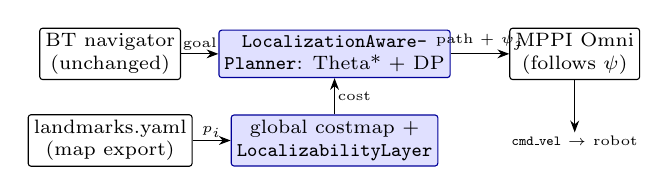
\begin{tikzpicture}[font=\scriptsize,
  box/.style={draw,rounded corners=1pt,align=center,inner sep=2pt,minimum height=6mm},
  ours/.style={box,fill=blue!12,draw=blue!60!black},
  lab/.style={font=\tiny,inner sep=1pt},
  >={Stealth[length=1.5mm]}]
\node[box]  (bt)    at (0,0)     {BT navigator\\(unchanged)};
\node[ours] (lap)   at (2.85,0)  {\texttt{LocalizationAware-}\\\texttt{Planner}: Theta* + DP};
\node[box]  (mppi)  at (5.9,0)   {MPPI Omni\\(follows $\psi$)};
\node[ours] (layer) at (2.85,-1.1) {global costmap +\\\texttt{LocalizabilityLayer}};
\node[box]  (lm)    at (0,-1.1)  {landmarks.yaml\\(map export)};
\node[lab]  (cmd)   at (5.9,-1.1) {\texttt{cmd\_vel} $\to$ robot};
\draw[->] (bt) -- node[lab,above]{goal} (lap);
\draw[->] (lap) -- node[lab,above]{path + $\psi_j$} (mppi);
\draw[->] (layer) -- node[lab,right]{cost} (lap);
\draw[->] (lm) -- node[lab,above]{$p_i$} (layer);
\draw[->] (mppi) -- (cmd);
\end{tikzpicture}
\caption{Integration. Blue: our plugins (C++); everything else is stock Nav2 Humble with the baseline BT.}
\label{fig:nav2}
\end{figure}

% =====================================================================
\section{Experiment}
% =====================================================================
\textbf{Modes.} \emph{Baseline}: stock Nav2 (\texttt{nav2\_params\_v2.yaml}, BT v3) unchanged. \emph{Active}: the same stack plus the two plugins (separate params file). \emph{Control}: the active stack with a \texttt{null} scorer and the layer disabled (\texttt{loc\_layer.enabled: false}; DP = forward prior); it isolates the effect of the stack itself (DP headings, PathAlign settings) from that of the scorer.
% src: _team/DECISIONS.md D-2, D-8 (control inherits offset_from_furthest 4: baseline<->control = stack, control<->active = method); _team/tasks/T-009_method_impl.md §5 v2 (RND-7 item 1)
\textbf{Scenario and protocol.} \texttt{shelves\_loop\_a}: from the spawn pose $(-2.0,-0.5)$ via $(2.6,-0.8)$ and $(-0.5,2.45)$ back to the start, 16.2\,m.
% src: navigation/src/al_eval/config/scenarios/shelves_loop_a.yaml (3 goals); 16.2 m: _team/final_inputs/summary_x4.md (path length GT 16.24/16.11/16.19 m)
Every run restarts the simulator, localization and Nav2 from a pristine copy of the map database, with the same spawn pose and a 0.6\,m nudge before the first goal (RTAB-Map otherwise initialises from the last pose stored in the database). Seeds 42--46; for each seed the three modes run back to back in a rotated order (interleaved); 15 runs per noise level.
% src: _team/DECISIONS.md D-2; FACTS.md 16.10 (spawn), 18.10 (DB re-initialisation); _team/final_inputs/T-010b_ENG.md "Setup" (seeds 42-46, interleaved per seed with rotated order, 15 runs per series, 30 in total)
A first run (T-010: 3 seeds, modes in blocks) is superseded: its real-time factor differed between modes (baseline 0.63, control 0.74), a confound; with interleaving the RTF is 0.75--0.78 in 26 of 30 runs in every mode.
% src: _team/final_inputs/07_results_draft.md §A L3 "Confound (ENG-35)" (RTF baseline 0.63 +- 0.02, control 0.74 +- 0.03); T-010b_ENG.md "Setup" (RTF 0.75-0.78 for 26/30 runs in every mode)
\textbf{Odometry noise.} Gazebo odometry is perfect, so drift is injected: a random walk whose variance grows with distance and rotation (default $\sigma_x\approx5$\,cm per 10\,m), 1\,\% scale error and 0.01\,rad/m yaw drift, scaled by a factor $k$, with the same seeds in all modes. $k=4$ was fixed before any active run by a pre-registered rule (D-5); $k=6$ is a stress level added after T-010. Yaw noise grows per radian turned, so the turning active mode receives more drift by design.
% src: _team/DECISIONS.md D-3 (rotation term penalises the turning mode, to be stated), D-5 (rule; result frozen x4, 18.10 15:50); navigation/src/al_odom_noise/config/odom_noise.yaml (defaults: k_xx 2.5e-4 m^2/m, scale_x/y 0.01, yaw_drift_per_m 0.01, k_rr 5.0e-4 rad^2/rad); x6 "added after T-010": 07_results_draft.md §B2 (D-9), 08_final_findings.md C4
% NOTE: the x4/x6 multiplier is applied by ENG's run script (eng/19_overnight_t010b.sh, not in this repo); which parameters it scales is not restated here.
\textbf{Metrics.} Ground truth = Gazebo pose, estimate = \texttt{map}$\to$\texttt{base\_link}. APE and RPE (translation, $xy$, RPE every 1\,m) with evo 1.38 and \emph{no alignment}, since Umeyama alignment hides drift.
% src: eval/README.md; FACTS.md 16.10 (evo 1.38, alignment hides drift: 0.173 -> 0.072 m on synthetic data)
Mechanism: share of the path with a marker in view ($\ge1$ accepted detection in the last 1\,s), longest arc without one, detections per metre. Secondary: \texttt{map}$\to$\texttt{odom} corrections, time, path length, rotation, goals reached.
% src: 07_results_draft.md §A L1 (path share metric, 1 s window, longest blind arc), §B3 (primary/secondary outcomes); eval/README.md §7 (summary.csv columns)
All series are cropped to [first goal start, last goal end] (start-up relocalization excluded), and \texttt{map}$\to$\texttt{odom} corrections are measured from the identity, since odometry starts at the ground-truth pose.
% src: eval/README.md §7 (T-011c: cropping on, --map-odom-ref zero by default); odom_noise.yaml (init_from_gt: true); summary_x4.md header (not aligned, window result.yaml, reference identity)
\textbf{Statistics} (fixed before the runs). The unit is a seed (one interleaved triple); we report the mean paired difference with its 95\,\% $t$-interval ($n=5$) and the number of seeds with that sign; no $p$-values. Primary: ${\times}4$; ${\times}6$ is descriptive.
% src: _team/final_inputs/07_results_draft.md §B (1 unit, 2 series, 5 t-interval df 4, 7 no p-values; written before T-010b)
\textbf{Pre-registered prediction.} The Python oracle replayed the scenario offline before any run (spec v2, path tracked exactly): a marker in view on 7\,\% of the path for the baseline and $\approx$60\,\% for the active mode (longest blind stretch 8.6 vs 3.7\,m). The layer leaves the loop\_a route unchanged, but bends a straight leg by 0.5\,m from $c_{\max}\approx120$; hence $c_{\max}=150$ and a separate route-lever demo (D-6: one run, seed 42, ${\times}4$, a straight leg at $y=-1.4$\,m below the marker rows).
% src: _team/predict_v2/prediction.md (T-011b v2): n_eff>=0.5 frac L 0.074 (baseline) vs 0.616 (active; s>=0.5: 0.604), longest gap 8.61 vs 3.66 m; c_max sweep: loop_a dL -0.0 % up to 80, -0.8 % at 160; straight-leg probe offset 0.53 m at c_max 120
% src (demo): _team/final_inputs/T-010b_ENG.md "D-6" (runs/d6_20261019_055924, seed 42, x4, shelves_south_wall.yaml, leg 2 planned straight line y = -1.4); DECISIONS.md D-6 option (b)

% =====================================================================
\section{Results}
% =====================================================================
% Text: RND final, _team/final_inputs/08_final_findings.md §3 "§5 Results" (verbatim; only the Table/Fig. references are added)
All 90 goals of the main experiment were reached (loop\_a, 5 seeds $\times$ 3 modes, modes interleaved per seed, odometry noise ${\times}4$ as pre-registered and ${\times}6$ as an added stress level).
% src: T-010b_ENG.md "Setup" (90/90 goals); summary_x4.md, summary_x6.md (goals reached 15/15 per mode)
The method changes what the robot sees, as predicted offline. The path share with a marker in view rose from 33\,\% to 66\,\% at ${\times}4$ (prediction 60\,\%; +32\,pp, 95\,\% CI [+29, +36], 5/5 seeds; Table~\ref{tab:results}, Fig.~\ref{fig:results}b), detections rose ${\times}4.7$ and the longest blind arc fell from 4.9 to 3.3\,m.
% src: 08_final_findings.md C1 (33 -> 66 %, +32 pp [+29, +36], 5/5, predicted 60 %, detections x4.7, blind arc 4.9 -> 3.3 m); 07_results_draft.md §D1; det/m 3.0 -> 14.1: summary_x4.md
The control (same stack, null scorer) stayed at baseline. When the planned route has no marker in view, the layer bends it into the marker band (Fig.~\ref{fig:results}a: 0.5\,m detour, 0\,$\to$\,69 detections, +2\,s).
% src: 08 C1 (control ~ baseline; path share 22 %, det/m 3.3: 07 §D3, summary_x4.md); 08 C2 / T-010b_ENG.md D-6 (y -1.24 ... -0.86, bends 0.54 m; detections 0 -> 69; +0.15 m, +2.1 s)
Accuracy at ${\times}4$ did not change measurably: APE RMSE $\Delta=-1.5$\,mm [$-6.2$, $+3.2$] (baseline 40\,mm), so the gain is at most 6\,mm.
% src: 08 C3 (-1.5 mm [-6.2, +3.2], 3/5; upper bound 6.2 mm ~ 16 %); baseline 0.040 m: summary_x4.md
At ${\times}6$ the estimates grow: APE RMSE $-4.8$\,mm [$-11.4$, $+1.8$], APE max $-22$\,mm (5/5), and the largest localization jump is 9\,cm smaller than in the control (5/5). The cost is +23\,\% (${\times}4$) to +30\,\% (${\times}6$) time.
% src: 08 C4 (APE RMSE -4.8 [-11.4, +1.8], 4/5; APE max -21.6 [-38.5, -4.7], 5/5), C5 (map->odom max step active - control -0.089 m [-0.163, -0.016], 5/5), C7 (time +8.2 s +23 % at x4, +12.1 s +30 % at x6, 5/5)

% =====================================================================
\section{Discussion, limitations, improvements}
% =====================================================================
% Text: RND final, _team/final_inputs/08_final_findings.md §3 "§6 Discussion" (verbatim)
On this map, lidar ICP bounds the error near 4\,cm. Landmark constraints are largely redundant, and the error does not drop while a marker is in view. The benefit of looking at markers shows up only as drift grows, consistent with markers acting as a backup when ICP corrections lag.
% src: 08 C8 [hypothesis] (active x4: APE 0.043 m with a marker in view vs 0.031 m without; effect appears only with more drift); baseline APE RMSE 40 / 54 mm: summary_x4.md, summary_x6.md
The control was slightly more accurate than the baseline at ${\times}4$ ($-2.7$\,mm), so part of any difference comes from heading-aware path following itself.
% src: 08 C6 (control - base APE RMSE -2.7 mm [-4.8, -0.6], 5/5)
Limitations: one scenario, 5 seeds, simulation; ${\times}6$ was added after the first run; the route demo is a single run; the detection model was fitted on one marker. Improvements: an uncertainty-gated heading term to cut the time cost, a lidar-degeneracy term in the scorer, and tests in ICP-poor corridors.
% src: 08 §3; FACTS.md 18.10 (ENG-10 detection model fitted on one marker); DECISIONS.md D-7 (lidar-degraded condition deferred)

% ---------------------------------------------------------------------
% Table 3: x4 summary from eval/summarize.py (_team/final_inputs/summary_table.tex = runs/t010b_20261019_055924/x4/summary/summary_table.tex, 7 rows)
% + row "Path with marker in view" + column "Delta active - base [95 % CI]" (08 §4, 07 §D3 "Table 2").
% Changes vs the generated file: APE in mm instead of m (0.040 m = 40 mm, same digits); std columns kept.
% Inlined (not \input) because of the extra row/column; eval_out/summary_table.tex is no longer read.
\begin{table}[t]
\centering\scriptsize
\setlength{\tabcolsep}{1.1pt}
\caption{Noise ${\times}4$ (primary): mean $\pm$ std over 5 seeds; $\Delta$: mean paired difference active $-$ baseline, 95\,\% $t$-interval. More metrics: repository.}
\label{tab:results}
\begin{tabular}{@{}lcccc@{}}
\toprule
Metric & baseline & active & control & $\Delta$ [95\,\% CI] \\
\midrule
% src: 08_final_findings.md §4 (33 / 66 / 22), C1 (+32 pp [+29, +36]); 07_results_draft.md §D1, §D3
Path with marker [\%] & 33 & 66 & 22 & $+32$\,[$+29$,\,$+36$] \\
% src: summary_table.tex rows (x4); Delta CIs: 07_results_draft.md §D3 "Table 2" line, 08 C3
APE RMSE [mm] & $40\!\pm\!2$ & $39\!\pm\!3$ & $37\!\pm\!1$ & $-1.5$\,[$-6.2$,\,$+3.2$] \\
APE max [mm] & $119\!\pm\!21$ & $117\!\pm\!12$ & $109\!\pm\!25$ & $-1.9$\,[$-31$,\,$+27$] \\
Detections per m & $3.0\!\pm\!0.8$ & $14.1\!\pm\!0.7$ & $3.3\!\pm\!0.7$ & $+11.1$\,[$+9.6$,\,$+12.6$] \\
Max $|$\texttt{map}$\to$\texttt{odom}$|$ [m] & $1.279\!\pm\!0.557$ & $1.083\!\pm\!0.299$ & $1.069\!\pm\!0.335$ & $-0.20$\,[$-0.96$,\,$+0.57$] \\
% src: time CI 08 C7 / 07 §D3; path length Delta -0.132 (5/5): summary_x4.md "Paired by seed" (no CI computed by RND)
Time [s] & $36.0\!\pm\!1.9$ & $44.2\!\pm\!2.0$ & $40.5\!\pm\!0.9$ & $+8.2$\,[$+6.9$,\,$+9.4$] \\
Path length [m] & $16.2\!\pm\!0.0$ & $16.1\!\pm\!0.1$ & $16.2\!\pm\!0.0$ & $-0.13$ (5/5) \\
Goals reached & 15/15 & 15/15 & 15/15 & -- \\
\midrule
% src: summary_x6.md (APE RMSE 0.054 / 0.049 / 0.053 m, APE max 0.160 / 0.138 / 0.159 m); 08 §4
\multicolumn{5}{@{}p{\linewidth}@{}}{${\times}6$ (stress): APE RMSE 54 / 49 / 53\,mm, APE max 160 / 138 / 159\,mm.} \\
\bottomrule
\end{tabular}
\end{table}
\vspace{-2pt}
\footnotesize
\begin{thebibliography}{9}\setlength{\itemsep}{0pt}
\bibitem{fif} Z.~Zhang, D.~Scaramuzza, ``Fisher Information Field: an Efficient and Differentiable Map for Perception-aware Planning,'' arXiv:2008.03324, 2020.
\bibitem{lwl} L.~Di~Giammarino et al., ``Learning Where to Look: Self-supervised Viewpoint Selection for Active Localization using Geometrical Information,'' arXiv:2407.15593, 2024.
\bibitem{ravpp} S.~Barlakas et al., ``Robot Active Vision-Based Path Planning for Localization Improvement in Indoor Environments,'' in Proc.\ IEEE/RSJ IROS, 2024.
\bibitem{actloc} J.~Li et al., ``ActLoc: Learning to Localize on the Move via Active Viewpoint Selection,'' in Proc.\ CoRL, 2025.
\end{thebibliography}
% src (references): first pages of the PDFs in docs/ (arXiv ids, IROS 2024 header, CoRL 2025 footer)

\end{document}
